\subsection{Back-end Support}\label{chap:kokkosBackend}

This section provides a practical insight into programming with Kokkos and the inner workings of the programming model library. Figure~\ref{fig:KokkosExample} shows am example application that algorithmically initializes an array to integers and includes several points of interests. Taking a closer look, the reader can observe the initialization and finalization of the Kokkos runtime library through the~\emph{Kokkos::initialize} and~\emph{Kokkos::finalize} method calls. Further the example shows the use of the~\emph{view} abstraction that represents a one-dimensional integer array of size~\emph{N}. The object carries the name~\emph{A} internally to facilitate tracing and debugging. In this example, a parallel\_for pattern object receives a range policy that is templated to the OpenMP execution space and takes~\emph{N} and a lambda expression as parameters. Vies behave as pointers and there a copy-semantic in the lambda expression is used in this case. Within the loop-body, the view object is accessed through the~\emph{()-operator}. It is up to the OpenMP execution space to provide performance implementations of the view, an efficient internal representation of the array and for the access operator for the underlying hardware architecture.

At compile time, the compiler generates the particular types, where in this case, the parallel\_for is types for the OpenMP execution space. At link time, the linker links this method to the corresponding parallel\_for implementation in the Kokkos library.

The implementation of the parallel\_for specific to the OpenMP execution space is shown in Figure~\ref{fig:KokkosExampleOMPBackEnd}. It shows the template argument of that class predefined to that execution space and shows how the~\emph{execute()} method calls the functor by calling ~\emph{exec\_range}. In can be seen that the Kokkos library relies on the back-end compiler to generate platform optimized, parallel code. 

\begin{figure}
\begin{small}
\begin{Verbatim}[frame=leftline]
int main(int argc, char* argv[]) {
  Kokkos::initialize(argc,argv);
  {
    int N = atoi(argv[1]);
    Kokkos::View<int*> a("A", N);  
    Kokkos::parallel_for(
    Kokkos::RangePolicy<Kokkos::OpenMP>(N,
    [=](const int & i)
    {
      a(i)=i*i;
    }); 
  }
  Kokkos::finalize();
}
\end{Verbatim}
\end{small}
\caption{An application written in Kokkos shows the use of a~\emph{view}-type and parallel for loop.}
\label{fig:KokkosExample}
\end{figure}



\begin{figure}
\begin{small}
\begin{Verbatim}[frame=leftline]
template <class FunctorType, class... Traits>
class ParallelFor<FunctorType, 
    ..., 
    Kokkos::OpenMP> {
  ...
private:
  ... cconst FunctorType& functor, 
  const Member i_beg,
  const Member i_end) 
  {
    for (Member i = i_beg; iwork < i_end; ++i){
      functor(t, i);
    }
  }

public:
  ...
  ... execute() const {(
  #pragma omp parallel num_threads(OpenMP::getPoolSize())
  {
    HostThreadTeamData& data=*(i->get_thread_data());
    ...
    range = data.get_work_partition();
    range(m_functor, range.first + m_policy.begin(),
    range.second + m_policy.begin());
  }
}

\end{Verbatim}
\end{small}
\caption{Library code giving an  insight into the impelemtnation of the OpenMP back-end shows ParallelFor class, its~\emph{execute} method and the internal use of the OpenMP pragma annotation.  internally gives an insight into the m maos how .}
\label{fig:KokkosExampleOMPBackEnd}
\end{figure}


\begin{figure}
\centerline{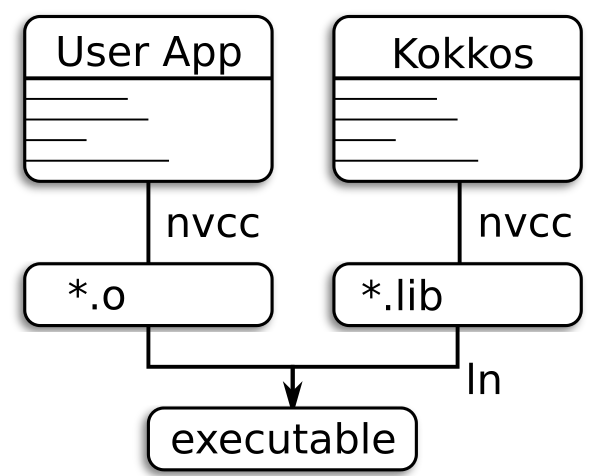
\includegraphics[width=0.3\textwidth]{img/Build.png}}
\caption{The compilation workflow includes the invocation of the platform compiler that is in charge to generate parallel   Building workflow}
\label{fig:workflow}
\end{figure}